\documentclass[11pt, a4paper]{article}
\usepackage[latin1]{inputenc}
\usepackage{pgfplots}
\usepackage{pgfplotstable}
\usepackage{float}
\pgfplotsset{width=0.85\textwidth ,compat=1.9}
\usepackage[dutch]{babel}
\usepackage{csquotes}
\usepackage{amsmath}
\usepackage{amsfonts}
\usepackage{amssymb}
\usepackage[backend=biber, style=numeric, citestyle=numeric-comp, sorting = none]{biblatex}
\author{Stef Tweepenninckx, r0677232}
\title{Practicum 1: Sorteeralgoritmes}


%define printtitle
\makeatletter
\def\printtitle{                 
    {\large \@title}} 
\makeatother

%define printauthor
\makeatletter                       
\def\printauthor{                  
    {\large \@author}}              
\makeatother

\begin{document}
\begin{titlepage}
\newcommand{\HRule}{\rule{\linewidth}{0.5mm}} 
\center 
\textsc{\LARGE Gegevensstructuren en algoritmen}\\[1.5cm] 
\HRule \\[0.4cm]

{\huge \bfseries \printtitle}\\[0.4cm] 
\HRule \\[0.4cm]

\Large \emph{Author:}\\
 \textsc{\printauthor}\\[3cm]

{\large \textsc{\today}}\\[3cm] 

\vfill 
\end{titlepage}

\section*{Inleiding}
\indent In dit verslag, dat ik moet maken voor het vak \emph{Gegevensstructuren en algoritmen}, zoek ik het antwoord op de onderzoeksvraag \emph{''Hoe effici\"ent zijn selection sort, insertion sort, en quicksort op random data?''} \\
\indent Om het antwoord op deze vraag heb ik de drie sorteeralgoritmes ge\"implementeerd en een aantal experimenten uitgevoerd. Deze experimenten worden verder beschreven.

\newpage
\section*{Aantal vergelijkingen}
\subsubsection*{Selection sort}
\paragraph{Werking selection sort} Selection sort is een van de meest eenvoudige sorteeralgoritmen. We doorlopen de array op zoek naar het kleinste element, waarna we dit element verwisselen met het eerste element van de array. Herhaal deze stappen tot we op het einde van de array zitten en de array gesorteerd is.
\paragraph{Verwachtingen} Bij selection sort verwachten we dat het aantal vergelijkingen, voor een array van N elementen, groeit volgens $\sim \frac{N^2}{2}$.
\paragraph{Experiment}\hspace{0pt}\\
De geplotte data (zie appendix) van de uitvoering van selection sort voor arrays met verschillend aantal elementen N:\\
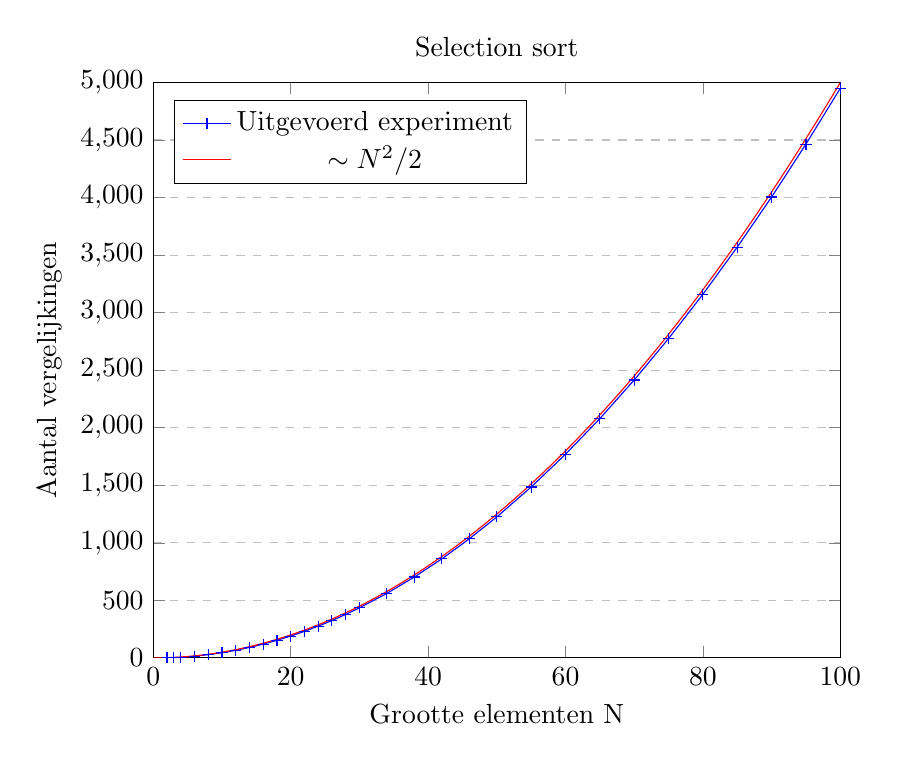
\begin{tikzpicture}
\begin{axis}[
    title={Selection sort},
    xlabel={Grootte elementen N},
    ylabel={Aantal vergelijkingen},
    xmin=0, xmax=100,
    ymin=0, ymax=5000,
    xtick={0,20,40,60,80,100},
    ytick={0,500,1000,1500,2000,2500,3000,3500,4000,4500,5000},
    legend pos=north west,
    ymajorgrids=true,
    grid style=dashed,
]
\addplot[
    color=blue,
    mark=+,
    ]
    coordinates {
    (2,1)(3,3)(4,6)(6,15)(8,28)(10,45)(12,66)(14,91)(16,120)(18,153)(20,190)(22,231)(24,276)(26,325)(28,378)(30,435)(34,561)(38,703)(42,861)(46,1035)(50,1225)(55,1485)(60,1770)(65,2080)(70,2415)(75,2775)(80,3160)(85,3570)(90,4005)(95,4465)(100,4950)
    };
    \legend{Uitgevoerd experiment};
\addplot [
    domain= 0:100, 
    samples=100, 
    color=red,
    ]
    {(x^2)/2};
    \addlegendentry{$\sim N^2 / 2$};
\end{axis}
\end{tikzpicture}
\paragraph{Conclusie experiment} Op bovenstaande grafiek kunnen we duidelijk zien dat de experimenten overeenkomen met de verwachte resultaten. De eventuele lichte afwijkingen kunnen we toeschrijven aan het feit dat we met random gegenereerde data zitten. Tussen deze random arrays kunnen arrays zitten die al (deels) gesorteerd zijn. Hierdoor hebben we dus minder vergelijkingen dan verwacht.\\
\indent We kunnen ook zien dat het aantal vergelijkingen zeer snel stijgt met het aantal elementen. Hieruit kunnen we afleiden dat selection sort ineffic\"ient is voor arrays met een groot aantal elementen.

\newpage
\subsubsection*{Insertion sort}
\paragraph{Werking insertion sort} Insertion sort is net als selection sort een eenvoudig sorteeralgoritme. We doorlopen de array van links naar rechts. Als het huidige element kleiner is dan een van de voorgaand elementen, verschuiven we het huidige element naar voor tot er geen kleiner element voor het huidige staat.
\paragraph{Verwachtingen} Bij insertion sort verwachten we dat het aantal vergelijkingen, voor een array van N elementen, groeit volgens $\sim \frac{N^2}{4}$. In het worst-case geval (een array die gesorteerd is van groot naar klein) groeit het aantal vergelijkingen volgens $\sim \frac{N^2}{2}$ 
\paragraph{Experiment}\hspace{0pt}\\
De geplotte data (zie appendix) van de uitvoering van insertion sort voor arrays met verschillend aantal elementen N:\\
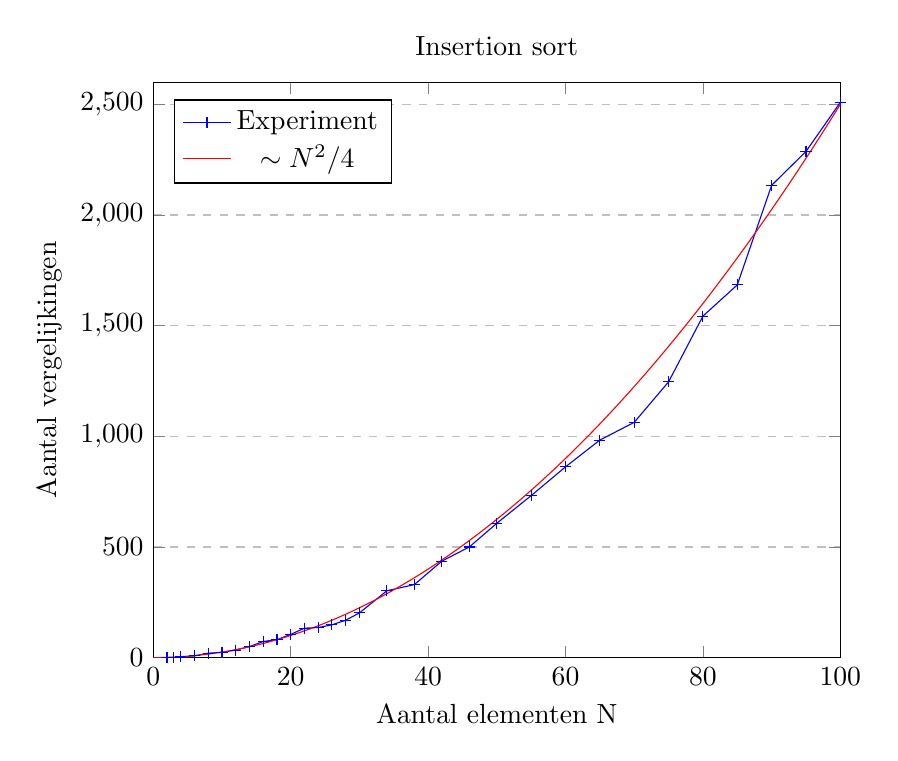
\begin{tikzpicture}
\begin{axis}[
    title={Insertion sort},
    xlabel={Aantal elementen N},
    ylabel={Aantal vergelijkingen},
    xmin=0, xmax=100,
    ymin=0, ymax=2600,
    xtick={0,20,40,60,80,100},
    ytick={0,500,1000,1500,2000,2500},
    legend pos=north west,
    ymajorgrids=true,
    grid style=dashed,
] 
\addplot[
    color=blue,
    mark=+,
    ]
    coordinates {(2,1)(3,1)(4,3)(6,8)(8,20)(10,24)(12,34)(14,50)(16,73)(18,81)(20,105)(22,133)(24,136)(26,148)(28,169)(30,202)(34,302)(38,330)(42,436)(46,500)(50,607)(55,732)(60,862)(65,983)(70,1063)(75,1246)(80,1543)(85,1684)(90,2134)(95,2287)(100,2509)
    };
    \legend{Experiment};
\addplot [
    domain= 0:100, 
    samples=100, 
    color=red,
    ]
    {(x^2)/4};
    \addlegendentry{$\sim N^2 / 4$};
\end{axis}
\end{tikzpicture}
\\
\paragraph{Conclusie experiment} Op bovenstaande grafiek kunnen we opnieuw zien dat de experimenten overeenkomen met de verwachte resultaten. De resultaten wijken wel meer af van de verwachte resultaten dan bij selection sort. Dit komt omdat het eventuele al (deels) gesorteerd zijn van de arrays, een grotere invloed heeft op het aantal vergelijkingen dan bij selection sort. Bij selection sort vergelijken we namelijk enkel met het eerste element, waar we bij insertion sort met elk voorgaand element vergelijken.
\indent Het aantal vergelijkingen stijgt ook bij insertion sort snel met het aantal elementen, maar minder dan bij selection sort. Hieruit kunnen we afleiden dat insertion sort een zeer goed algoritme is voor arrays met weinig elementen. Daarom wordt insertion sort vaak gebruikt als cutoff bij quicksort indien er weinig elementen te sorteren zijn.

\newpage
\subsubsection*{Quicksort}
\paragraph{Werking quicksort} Quicksort is een recursief sorteeralgoritme en daardoor iets minder eenvoudig dan voorgaande. We kiezen een pivot, meestal het 1e element, en vergelijken alle andere elementen uit de array hiermee. Zo delen we de array op in 3 delen: de pivot, elementen kleiner dan de pivot, en elementen groter dan de pivot. Dit herhalen we dan op de 2 deelarrays, enz.
\paragraph{Verwachtingen} Bij quicksort verwachten we dat het aantal vergelijkingen, voor een array van N elementen, groeit volgens $\sim 1.39nlg(n)$. 
\paragraph{Experiment}\hspace{0pt}\\
De geplotte data (zie appendix) van de uitvoering van quicksort voor arrays met verschillend aantal elementen N:\\
%TODO eventueel extra quicksort
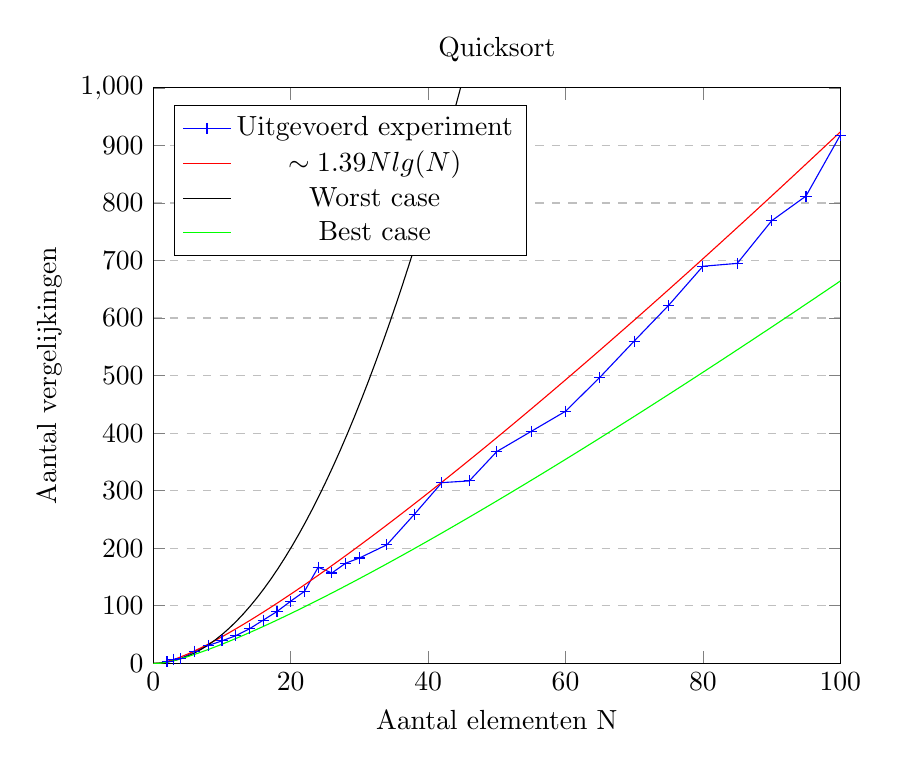
\begin{tikzpicture}
\begin{axis}[
    title={Quicksort },
    xlabel={Aantal elementen N},
    ylabel={Aantal vergelijkingen},
    xmin=0, xmax=100,
    ymin=0, ymax=1000,
    xtick={0,20,40,60,80,100},
    ytick={0,100,200,300,400,500,600,700,800,900,1000},
    legend pos=north west,
    ymajorgrids=true,
    grid style=dashed,
]
 
\addplot[
    color=blue,
    mark=+,
    ]
    coordinates {
	(2,3)(3,7)(4,8)(6,21)(8,31)(10,39)(12,48)(14,60)(16,75)(18,90)(20,108)(22,125)(24,167)(26,157)(28,174)(30,183)(34,206)(38,259)(42,314)(46,317)(50,368)(55,403)(60,438)(65,497)(70,560)(75,622)(80,690)(85,695)(90,769)(95,812)(100,918)
    };
    \legend{Uitgevoerd experiment};

\addplot [
    domain= 0:100, 
    samples=100, 
    color=red,
    ]
    {1.39*x*(log2(x))};
    \addlegendentry{$\sim 1.39Nlg(N)$}; 

\addplot [
    domain= 0:100, 
    samples=100, 
    color=black,
    ]
    {(x^2)/2};
    \addlegendentry{Worst case}; 
    
\addplot [
    domain= 0:100, 
    samples=100, 
    color=green,
    ]
    {x*(log2(x))};
    \addlegendentry{Best case}; 
\end{axis}
\end{tikzpicture}
\paragraph{Conclusie experiment} De resultaten van dit experiment komen overeen met de verwachte waarden. Opnieuw zijn er aantal lichte afwijkingen, maar ze bevinden zich mooi tussen de best en worst case van quicksort. De reden van afwijking bij quicksort is de keuze van de pivot, deze deelt de array niet altijd perfect in twee en dit kan leiden tot meer of minder vergelijkingen dan verwacht.


\subsection*{Algemene conclusie 1}
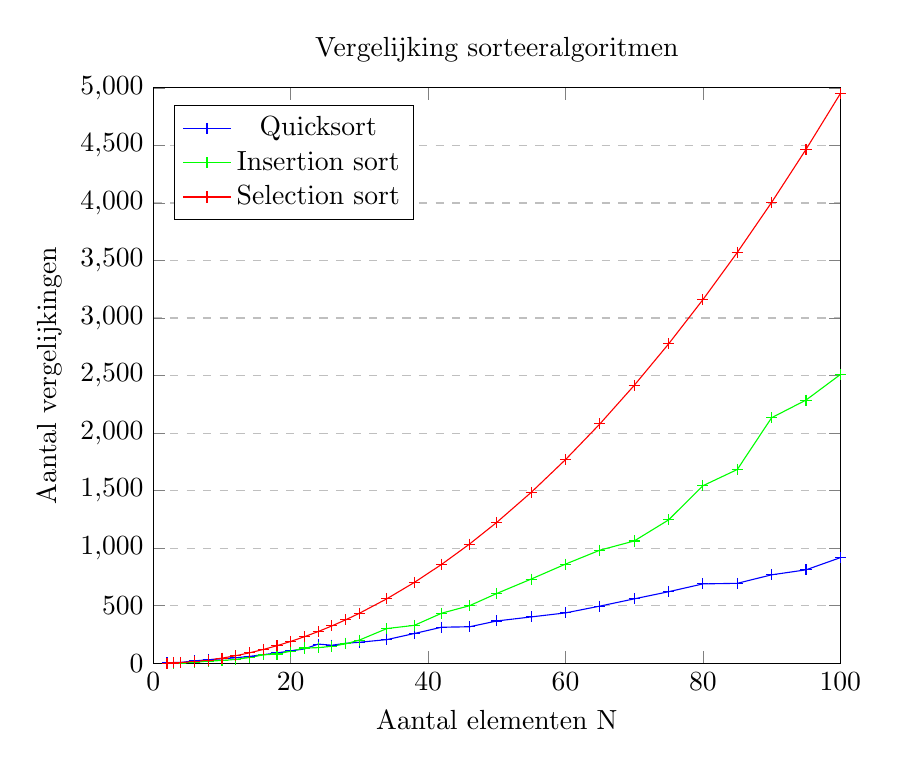
\begin{tikzpicture}
\begin{axis}[
    title={Vergelijking sorteeralgoritmen},
    xlabel={Aantal elementen N},
    ylabel={Aantal vergelijkingen},
    xmin=0, xmax=100,
    ymin=0, ymax=5000,
    xtick={0,20,40,60,80,100},
    ytick={0,500,1000,1500,2000,2500,3000,3500,4000,4500,5000},
    legend pos=north west,
    ymajorgrids=true,
    grid style=dashed,
]
 
\addplot[
    color=blue,
    mark=+,
    ]
    coordinates {
	(2,3)(3,7)(4,8)(6,21)(8,31)(10,39)(12,48)(14,60)(16,75)(18,90)(20,108)(22,125)(24,167)(26,157)(28,174)(30,183)(34,206)(38,259)(42,314)(46,317)(50,368)(55,403)(60,438)(65,497)(70,560)(75,622)(80,690)(85,695)(90,769)(95,812)(100,918)
    };
    \legend{Quicksort};
\addplot[
    color=green,
    mark=+,
    ]
    coordinates {(2,1)(3,1)(4,3)(6,8)(8,20)(10,24)(12,34)(14,50)(16,73)(18,81)(20,105)(22,133)(24,136)(26,148)(28,169)(30,202)(34,302)(38,330)(42,436)(46,500)(50,607)(55,732)(60,862)(65,983)(70,1063)(75,1246)(80,1543)(85,1684)(90,2134)(95,2287)(100,2509)
    };
    \addlegendentry{Insertion sort};
\addplot[
    color=red,
    mark=+,
    ]
    coordinates {
    (2,1)(3,3)(4,6)(6,15)(8,28)(10,45)(12,66)(14,91)(16,120)(18,153)(20,190)(22,231)(24,276)(26,325)(28,378)(30,435)(34,561)(38,703)(42,861)(46,1035)(50,1225)(55,1485)(60,1770)(65,2080)(70,2415)(75,2775)(80,3160)(85,3570)(90,4005)(95,4465)(100,4950)
    };
    \addlegendentry{Selection sort};
\end{axis}
\end{tikzpicture}\\
Zoals we duidelijk kunnen zien is quicksort het meest effici\"ente algoritme voor arrays met een groot aantal elementen. Bij een klein aantal elementen, $<20$, ligt het aantal vergelijkingen echter heel dicht bij elkaar. Vooral bij insertion sort en quicksort is het verschil zeer klein. Zoals eerder gezegd is dit een van de redenen dat insertion sort soms gebruikt wordt als cutoff bij quicksort voor een klein aantal elementen.


\newpage
\section*{Doubling ratio}
\subsection*{Insertion sort}
\begin{table}[H]
\centering
\label{my-label}
\begin{tabular}{|llll|}
\hline
\multicolumn{1}{|l|}{\textbf{N}} & \multicolumn{1}{l|}{\textbf{Tijd (milliseconden)}} & \multicolumn{1}{l|}{\textbf{ratio}} & \textbf{lg ratio} \\ \hline
1000                             & 15                                                 & -                                   & -                 \\
2000                             & 28                                                 & 1.9                                 & 0.93              \\
4000                             & 41                                                 & 1.5                                 & 0.58              \\
8000                             & 96                                                 & 2.3                                 & 1.20              \\
16000                            & 355                                                & 3.7                                 & 1.89              \\
32000                            & 1049                                               & 3                                   & 1.58              \\
64000                            & 4861                                               & 4.6                                 & 2.20              \\
128000                           & 19269                                              & 4                                   & 2                 \\ \hline
\end{tabular}
\caption{Doubling ratio insertion sort}
\end{table}

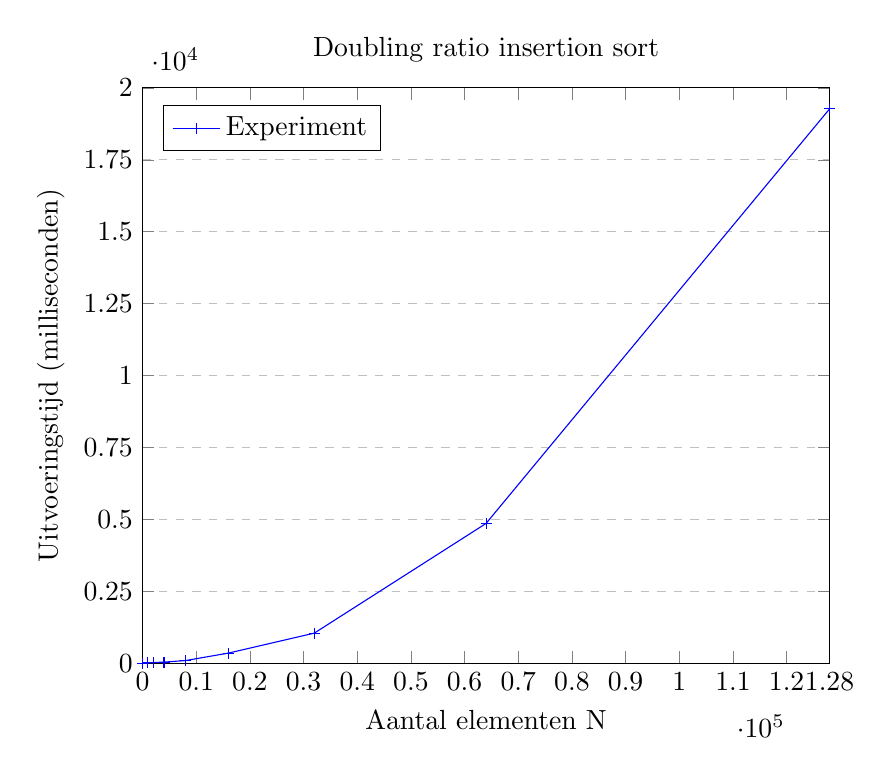
\begin{tikzpicture}
\begin{axis}[
    title={Doubling ratio insertion sort},
    xlabel={Aantal elementen N},
    ylabel={Uitvoeringstijd (milliseconden)},
    xmin=0, xmax=128000,
    ymin=0, ymax=20000,
    xtick={0,10000,20000,30000,40000,50000,60000,70000,80000,90000,100000,110000,120000,128000},
    ytick={0,2500,5000,7500,10000,12500,15000,17500,20000},
    legend pos=north west,
    ymajorgrids=true,
    grid style=dashed,
]
 
\addplot[
    color=blue,
    mark=+,
    ]
    coordinates {(0,0)(1000,15)(2000,28)(4000,41)(8000,96)(16000,355)(32000,1049)(64000,4861)(128000,19269)
    };
    \legend{Experiment};

\end{axis}
\end{tikzpicture}




\subsection*{Quicksort}
\begin{table}[H]
\centering
\label{my-label}
\begin{tabular}{|llll|}
\hline
\multicolumn{1}{|l|}{\textbf{N}} & \multicolumn{1}{l|}{\textbf{Tijd (milliseconden)}} & \multicolumn{1}{l|}{\textbf{ratio}} & \textbf{lg ratio} \\ \hline
1000                             & 1                                                  & -                                   & -                 \\
2000                             & 2                                                  & 2                                   & 1                 \\
4000                             & 3                                                  & 1.5                                 & 0.58              \\
8000                             & 5                                                  & 1.7                                 & 0.77              \\
16000                            & 9                                                  & 1.8                                 & 0.85              \\
32000                            & 15                                                 & 1.7                                 & 0.77              \\
64000                            & 29                                                 & 1.9                                 & 0.93              \\
128000                           & 40                                                 & 1.4                                 & 0.49              \\ \hline
\end{tabular}
\caption{Doubling ratio quicksort}
\end{table}

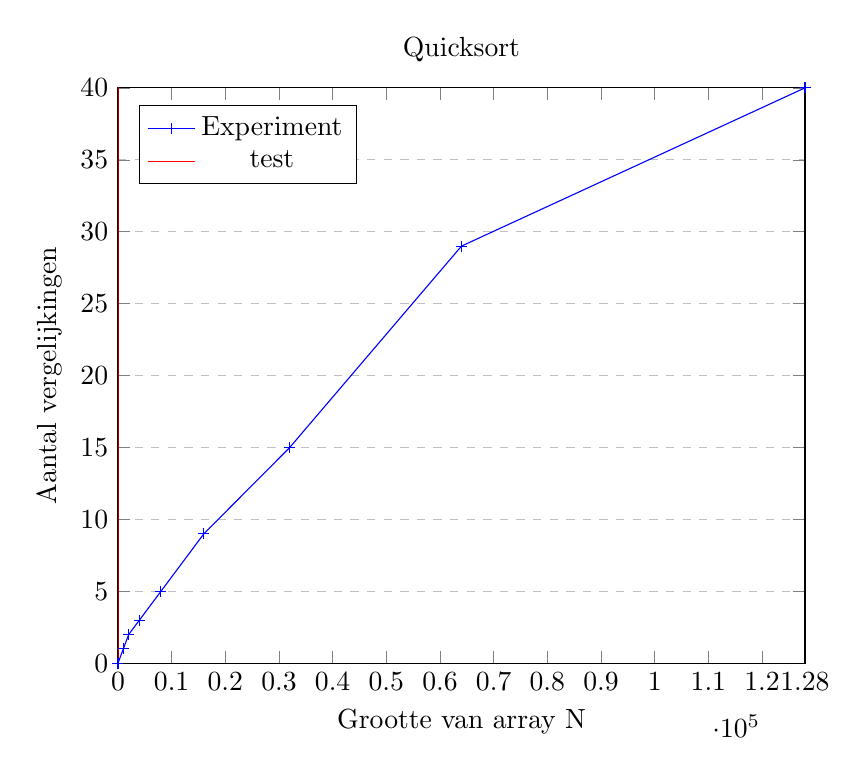
\begin{tikzpicture}
\begin{axis}[
    title={Quicksort},
    xlabel={Grootte van array N},
    ylabel={Aantal vergelijkingen},
    xmin=0, xmax=128000,
    ymin=0, ymax=40,
    xtick={0,10000,20000,30000,40000,50000,60000,70000,80000,90000,100000,110000,120000,128000},
    ytick={0,5,10,15,20,25,30,35,40},
    legend pos=north west,
    ymajorgrids=true,
    grid style=dashed,
]
 
\addplot[
    color=blue,
    mark=+,
    ]
    coordinates {(0,0)(1000,1)(2000,2)(4000,3)(8000,5)(16000,9)(32000,15)(64000,29)(128000,40)
    };
    \legend{Experiment};

\addplot [
    domain= 0:100, 
    samples=100, 
    color=red,
    ]
    {1.39*x*(log2(x))};
    \addlegendentry{test};
	
\end{axis}
\end{tikzpicture}

\pgfplotstableread{
9.966 0
10.966 1
11.966 1.585
12.966 2.322
13.966 3.170
14.966 3.907
15.966 4.858
16.966 5.322

}\datatable


\pgfplotstableread{
X Y
1000 2
2000 4
4000 6
8000 12
16000 14
32000 30
64000 54
128000 63
}\datatable

\begin{tikzpicture}
\begin{axis}[legend pos=outer north east]
\addplot [only marks, mark = *] table {\datatable};
\addplot [thick, red] table[
    y={create col/linear regression={y=Y}}
] % compute a linear regression from the input table
{\datatable};

\addplot [
    domain= 0:100, 
    samples=100, 
    color=blue,
    ]
    {1.39*x*(log2(x))};
\addlegendentry{$y(x)$}
\addlegendentry{%
$\pgfmathprintnumber{\pgfplotstableregressiona} \cdot x
\pgfmathprintnumber[print sign]{\pgfplotstableregressionb}$}
\end{axis}
\end{tikzpicture}
\end{document}
